\section{Actividad 2: Curva Característica de un Diodo}

 \subsection{Objetivo:}
 Realizar mediciones de corrientes y tensiones de los diodos rectificadores tanto
de Silicio como el de Germanio. Identificar principalmente el codo de conmutación entre el
estado de bloqueo a conducción y comparar estos datos con las especificaciones del
fabricante.


\subsection{Simulacion de Polarización en Directa:}

Primero implementamos el siguiente circuido en el simulador LTSpice:

\begin{figure}[ht!]
    \centering
    \begin{circuitikz}[american, scale=1.3, transform shape]
        \draw
        (0,0) to[battery, l=$V_1$] (0,3)
        (0,3) to[R, l=$R_1$] (2.8,3)
        (2.8,3) to[D, l_=$D_1$] (2.8,0)
        (2.8,0) -- (0,0)
        ;
        % Add ground at (0,0)
        \draw (0,0) node[ground]{};
    \end{circuitikz}
    \caption{}
\end{figure}

El circuito completo con sus respectivos valores es el siguiente:\\

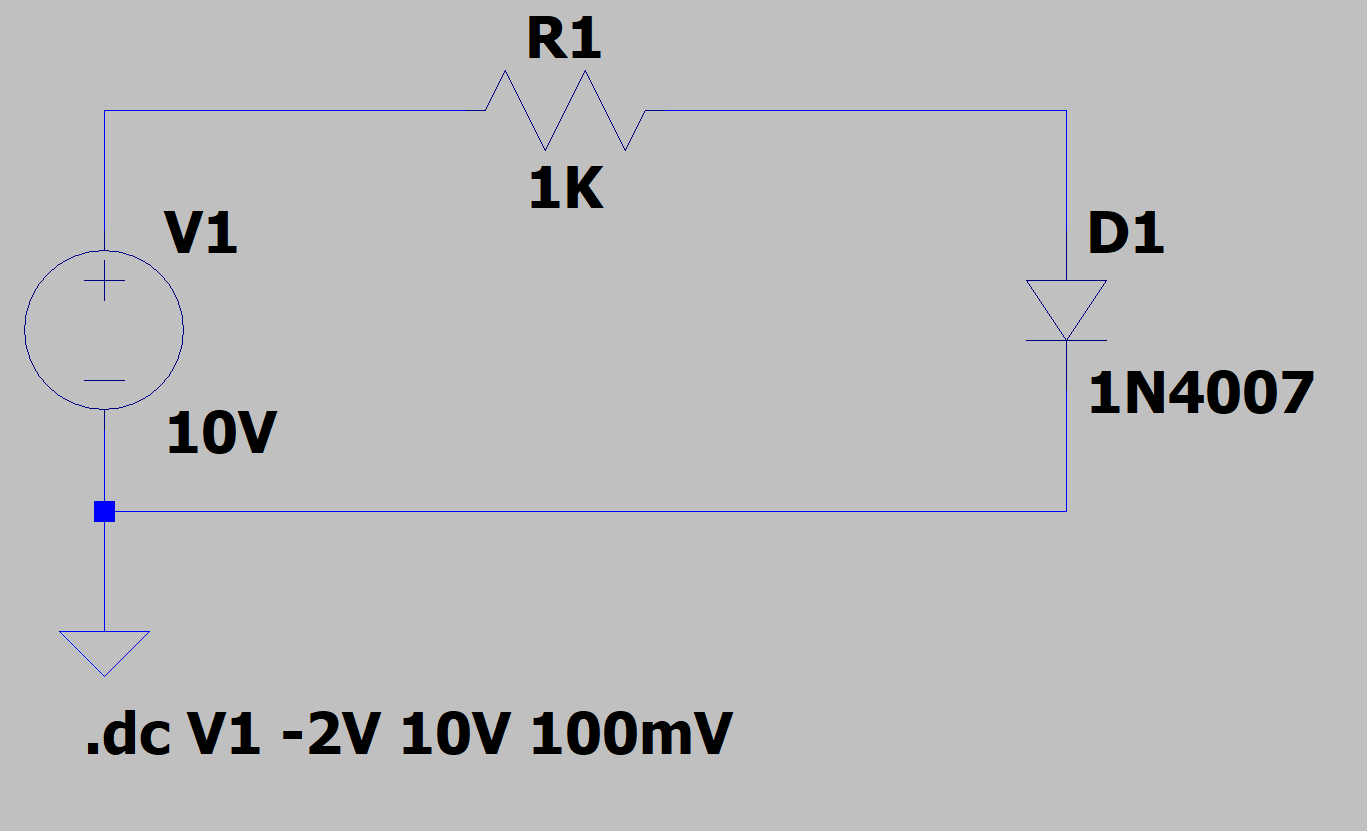
\includegraphics[width=9.3cm]{imagenes/Circuito1.png}\\

Luego de simular el circuito, obtenemos la siguiente curva característica:

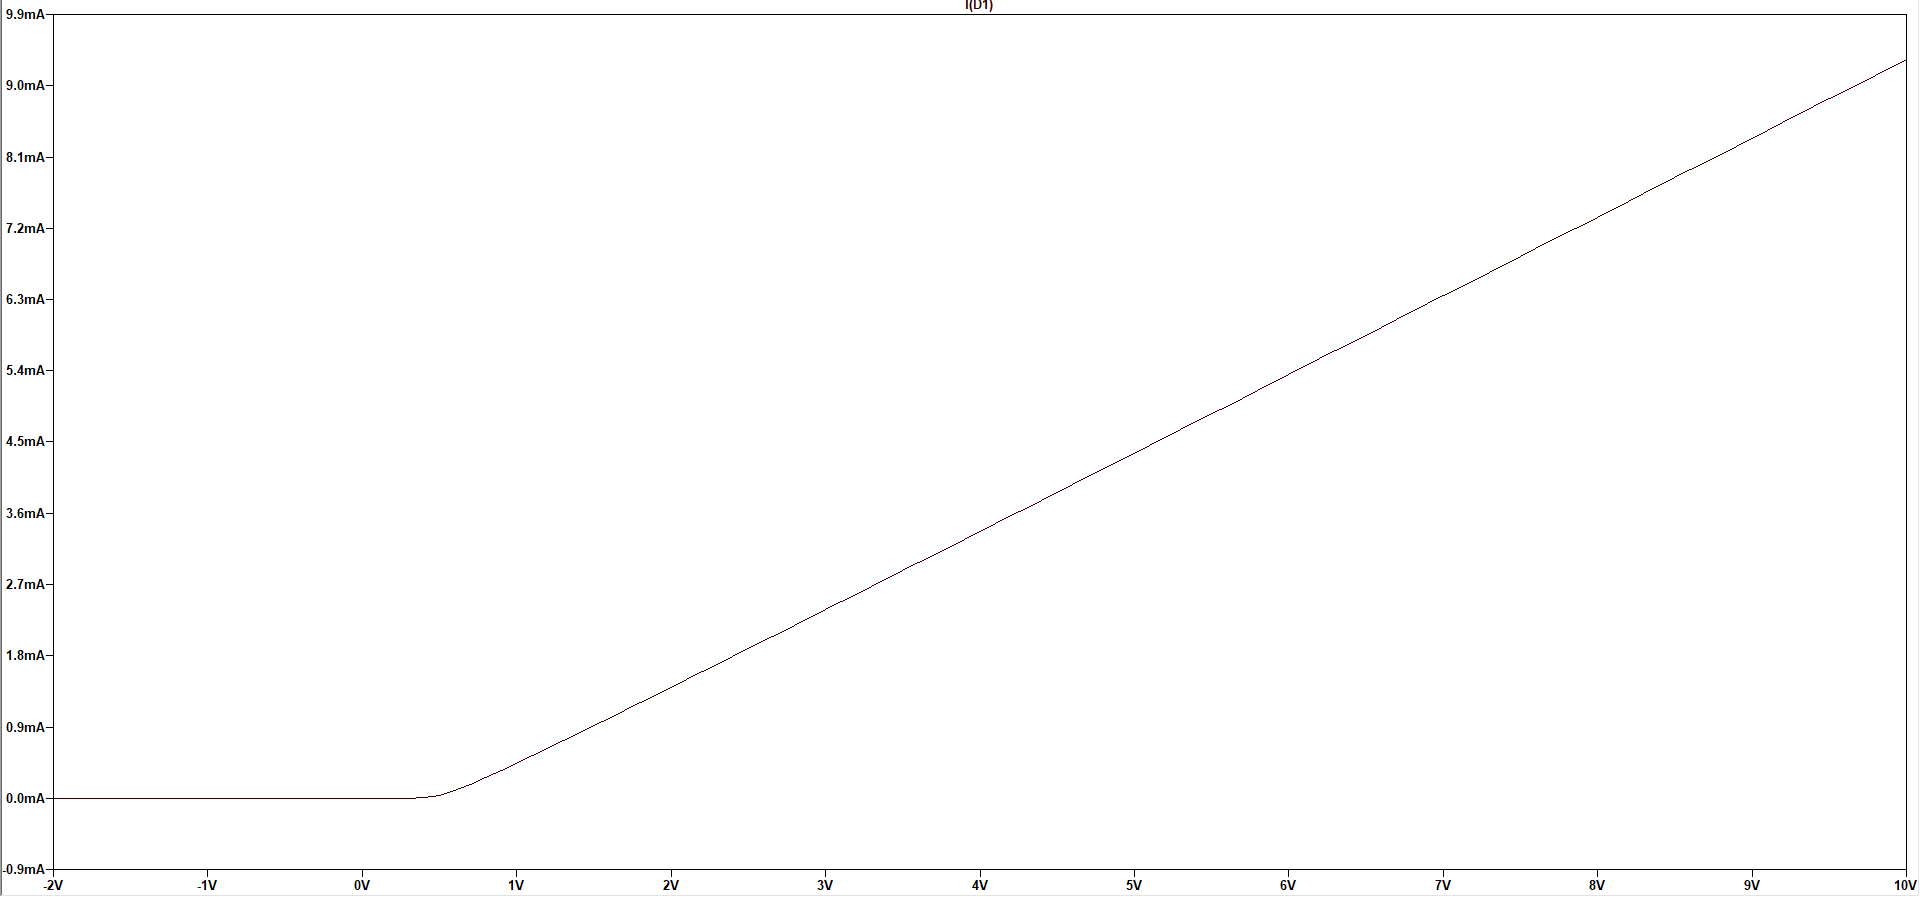
\includegraphics[width=9cm]{imagenes/simulacion11.png}\\

Ahora repetimos el proceso para el diodo de germanio, obteniendo el siguiente circuito:

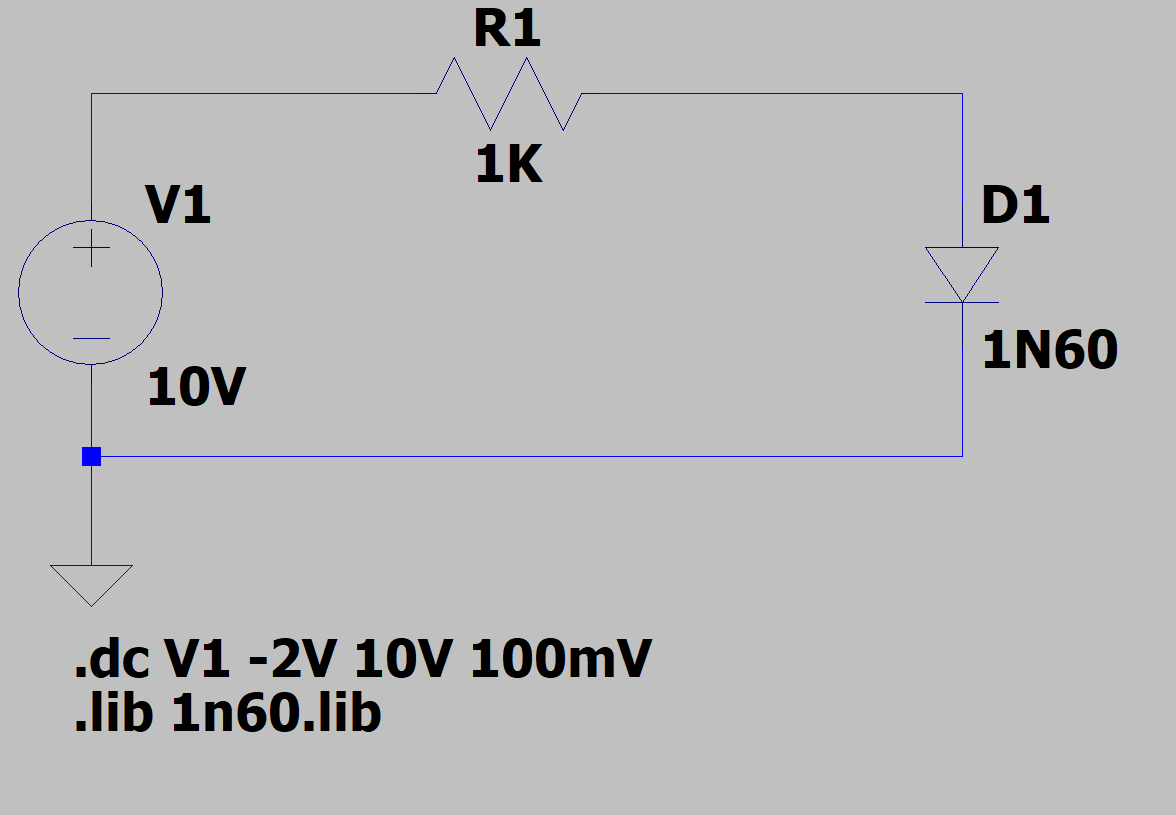
\includegraphics[width=8cm]{imagenes/Circuito2.png}\\

Y la curva característica:

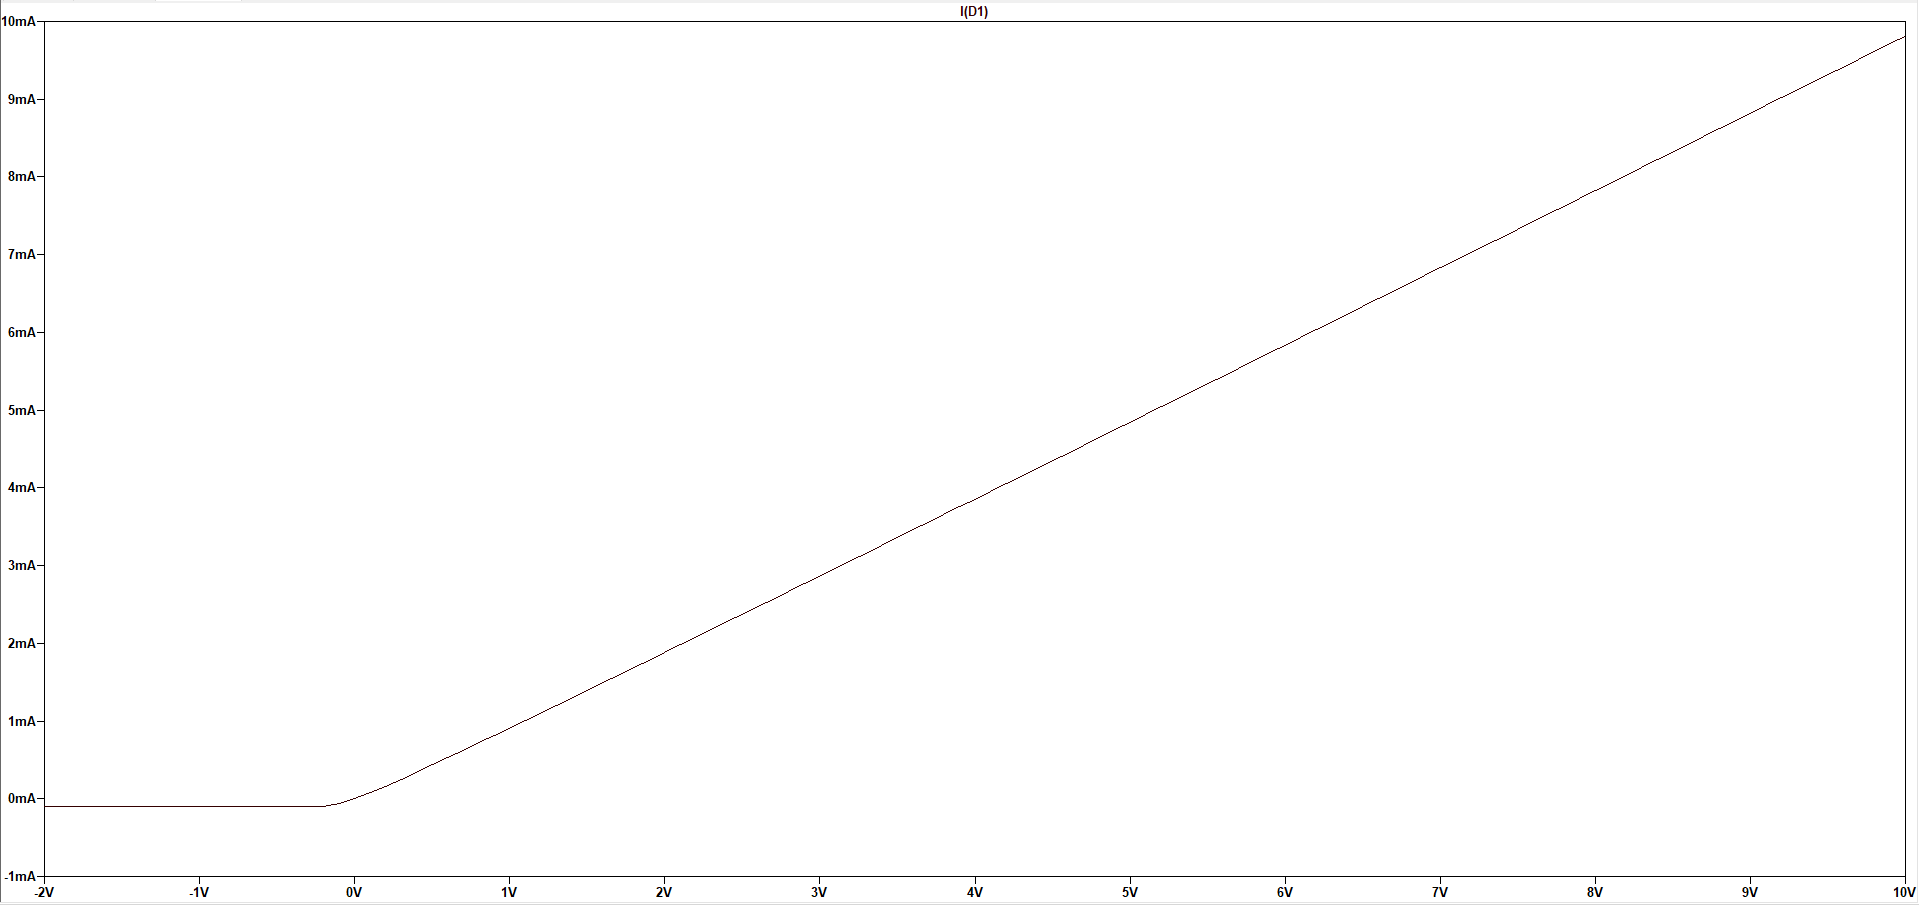
\includegraphics[width=8.2cm]{imagenes/simulacion2.png}\\

\subsection{Conslusiones de Polarizacion en Directa:}

Podemos concluir con que el diodo de germanio comienza a conducir a un voltaje menor que el de silicio, siendo este último de 0.7V y el primero de 0.3V aproximadamente. 


\subsection{Simulacion de Polarización en Inversa:}

Para la polarizacion en inversa debemos conocer el voltaje de ruptura del diodo, en el caso del 1N4007 es de 1000V y el del 1N60 es de 40V. Por lo que configuramos el simulador para obtener valores que superen esos:

\vspace{1cm}

\paragraph{Diodo de Silicio 1N4007:}

Circuito:
\vspace{0.5cm}

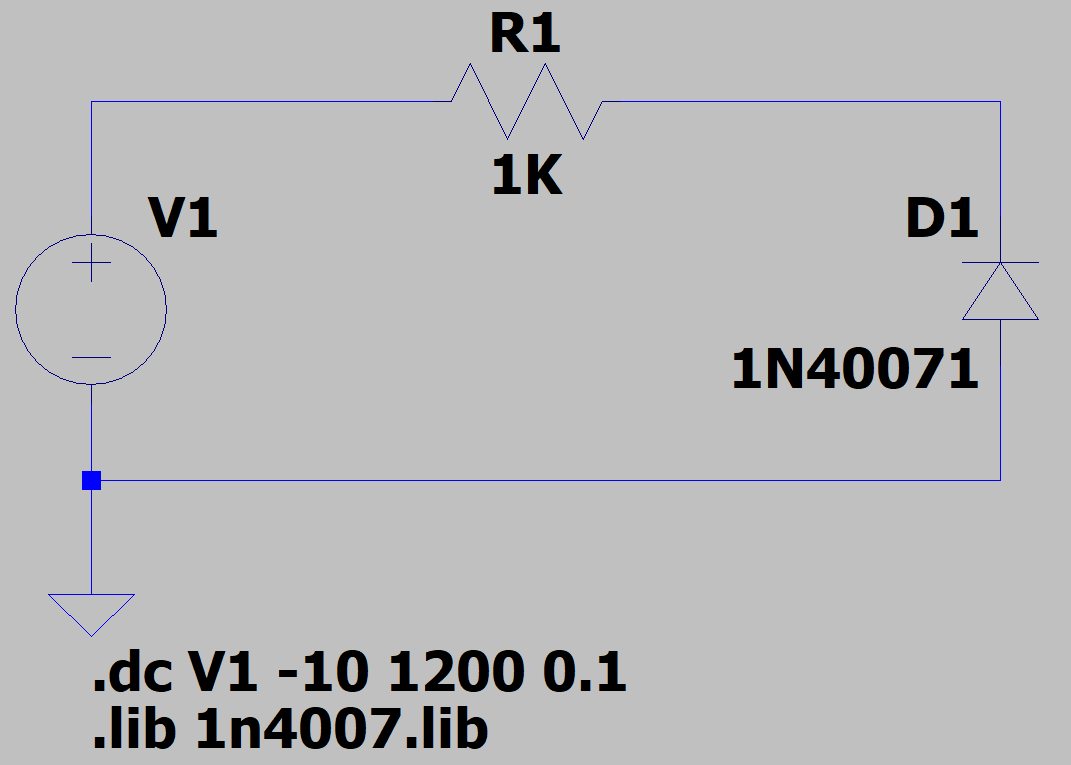
\includegraphics[width=8cm]{imagenes/Circuito3.PNG}

\vspace{0.5cm}

Simulación:

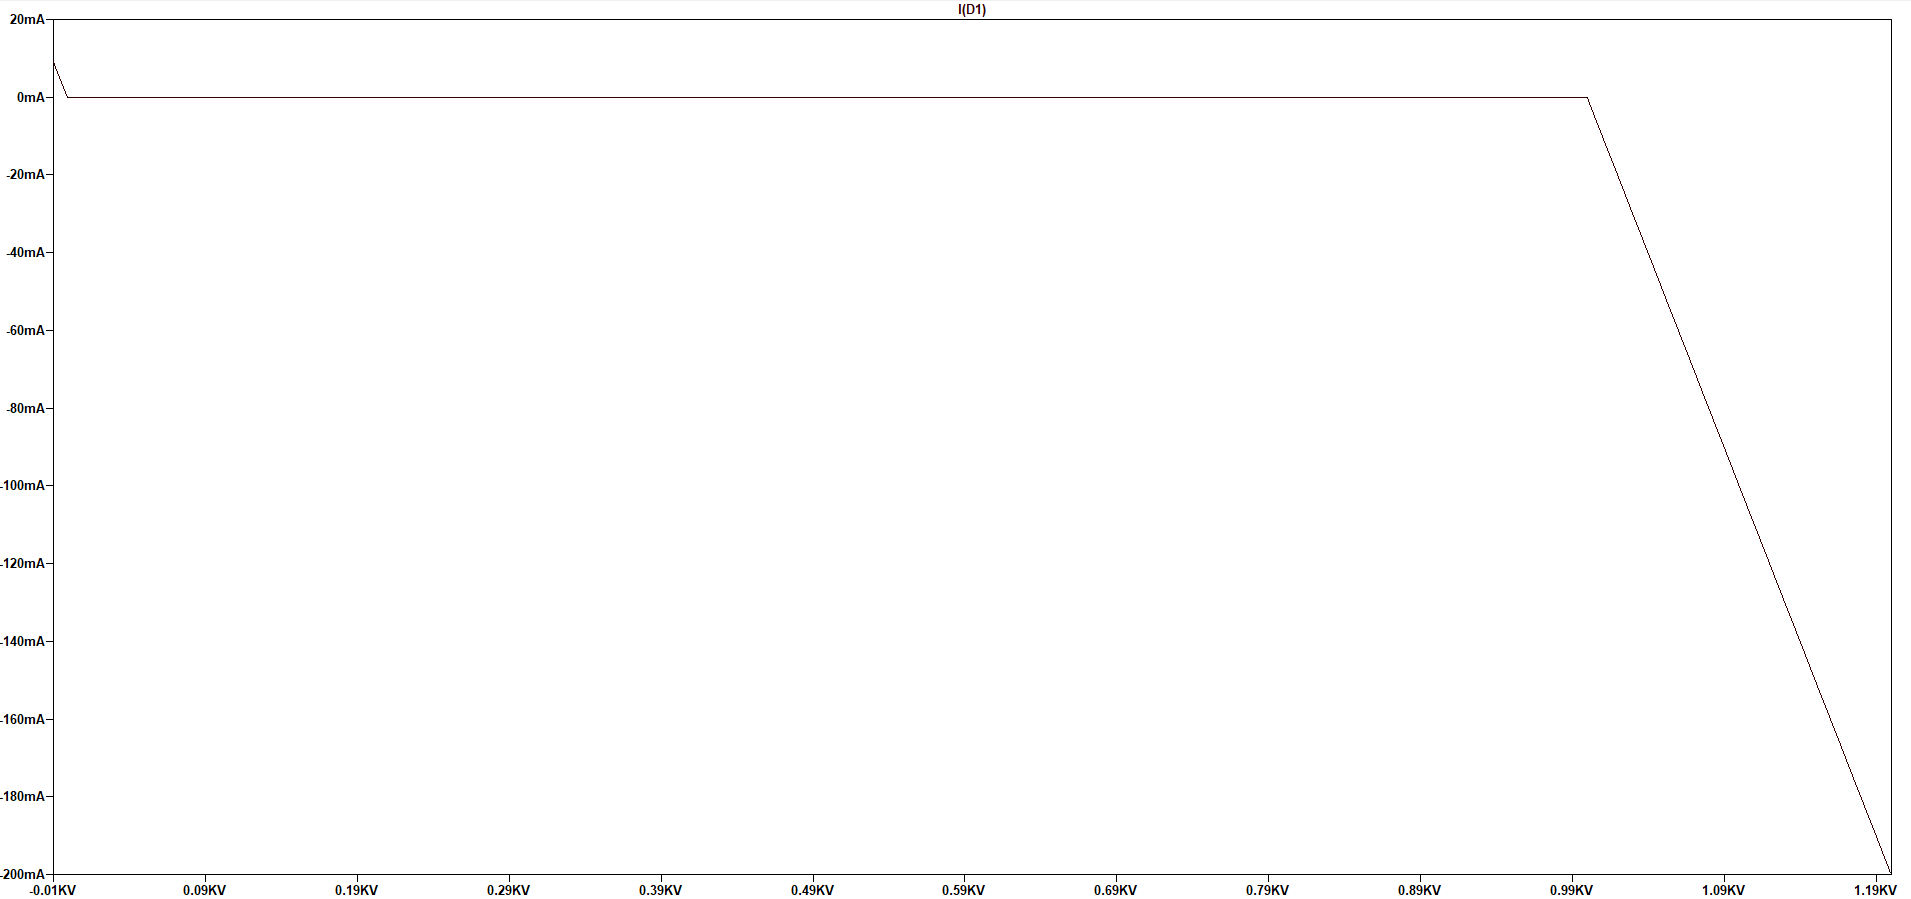
\includegraphics[width=8.2cm]{imagenes/simulacion3.png}\\

\paragraph{Diodo de Germanio 1N60:}

Circuito:

\vspace{0.5cm}

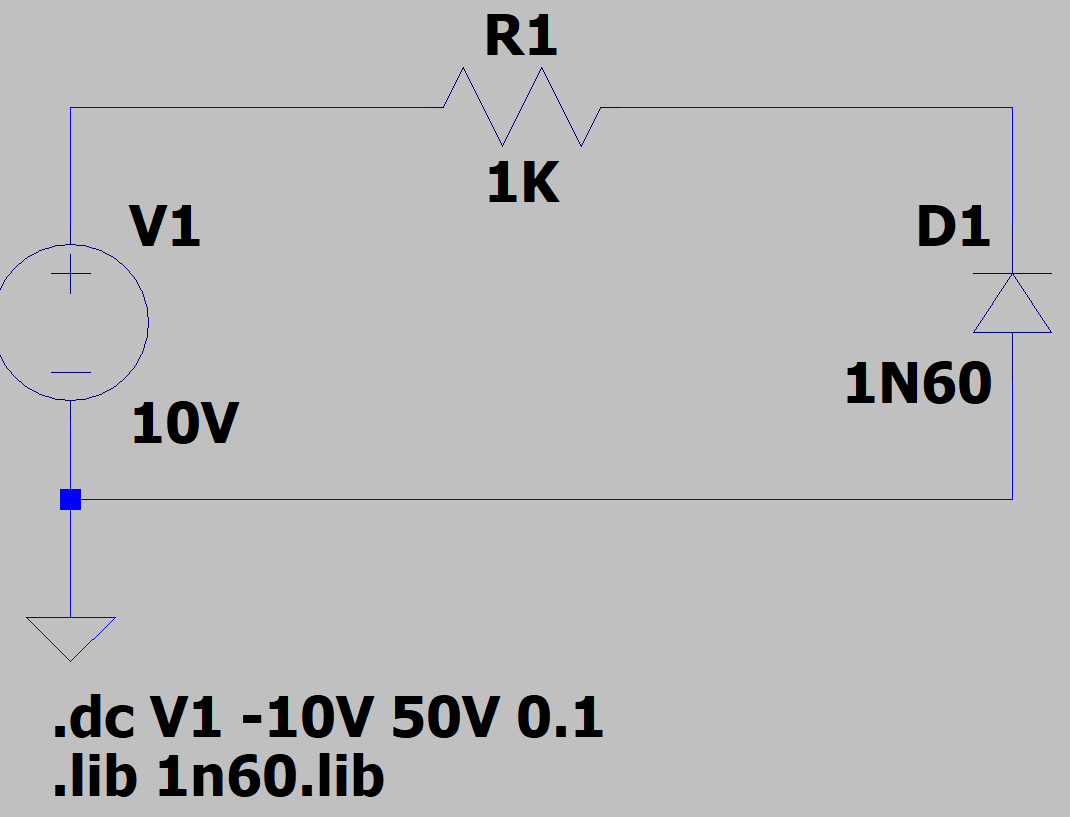
\includegraphics[width=8cm]{imagenes/Circuito4.png}\\

\vspace{0.5cm}

Simulación:

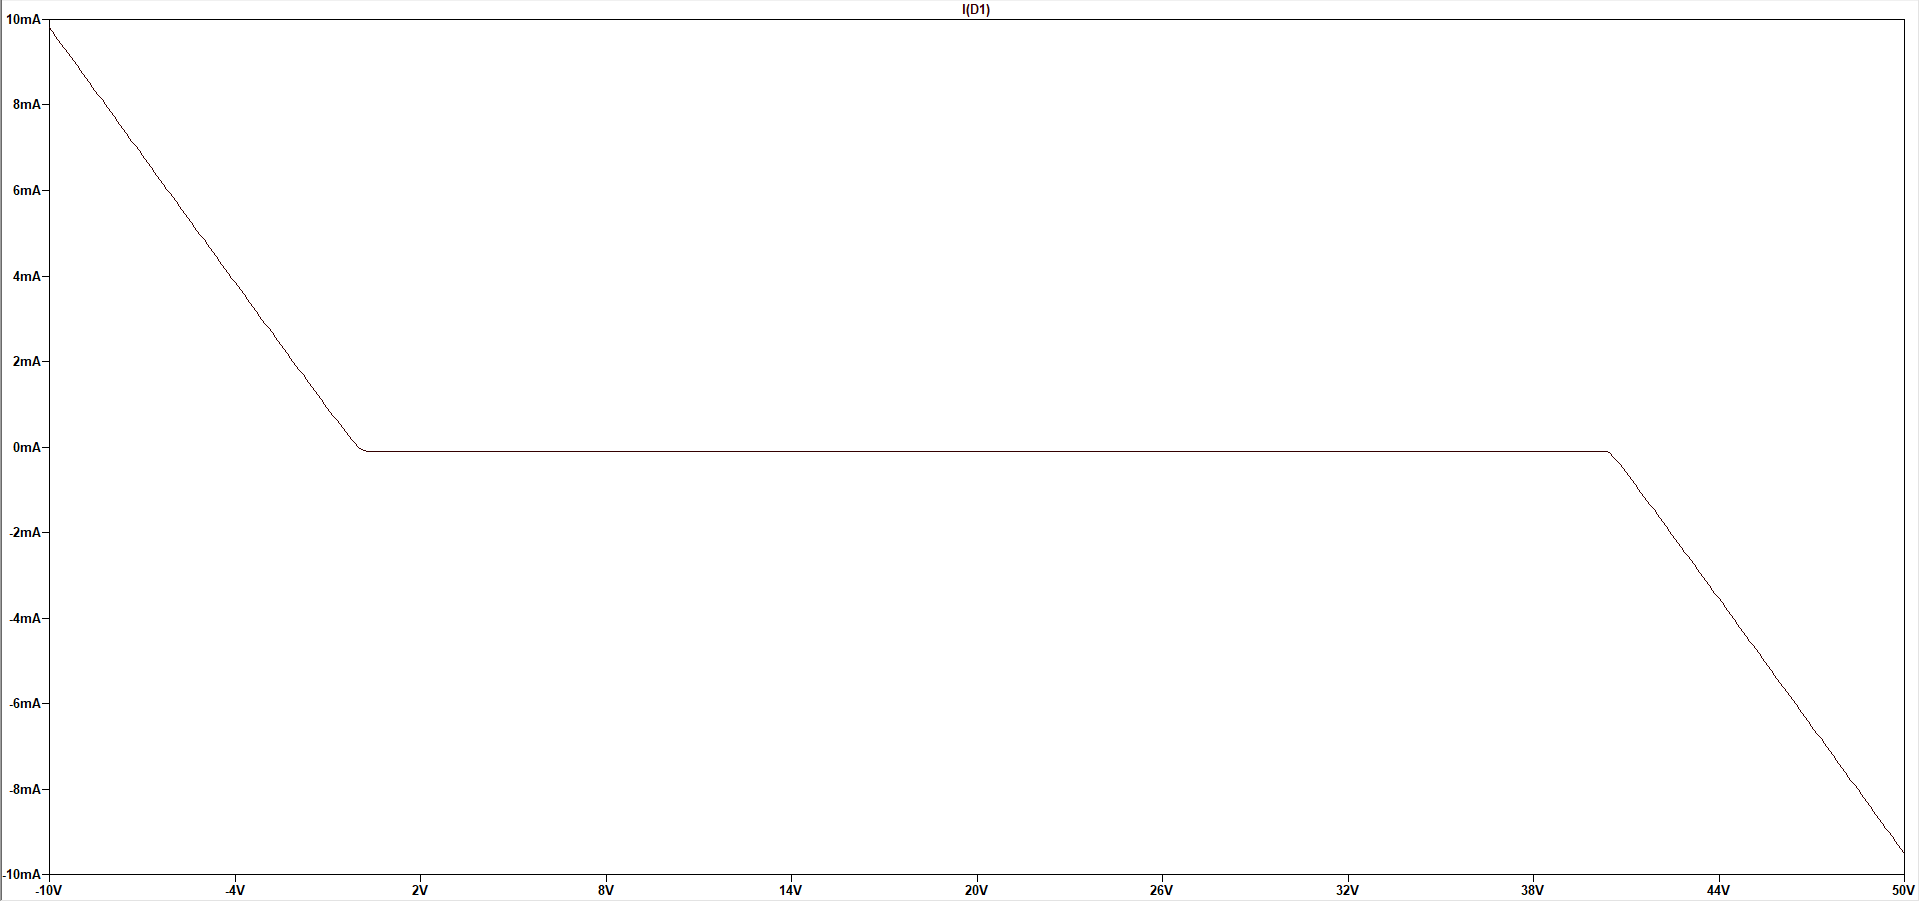
\includegraphics[width=8.2cm]{imagenes/simulacion4.png}\\

\subsection{Conclusiones de Polarizacion en Inversa:}

Al igual que el caso anterior, hay diferencias entre ambos diodos, el de germanio entra en ruptura a un voltaje mucho menor que el silicio, siendo este de 40V y 1000V respectivamente.


\subsection{Laboratorio:}

\subsubsection*{Materiales}

\begin{itemize}
    \item Un diodo de silicio (ej. 1N4007) , otro de germanio (ej. 1N60) y resistencia de 1k$\Omega$ $\frac{1}{8}$ o $\frac{1}{4}$ W.
    \item Dos multímetros (voltímetro y amperímetro µA).
    \item Fuente de alimentación variable.
    \item Protoboard.
\end{itemize}

\subsection*{Circuito experimental}

\begin{figure}[H]
    \centering
    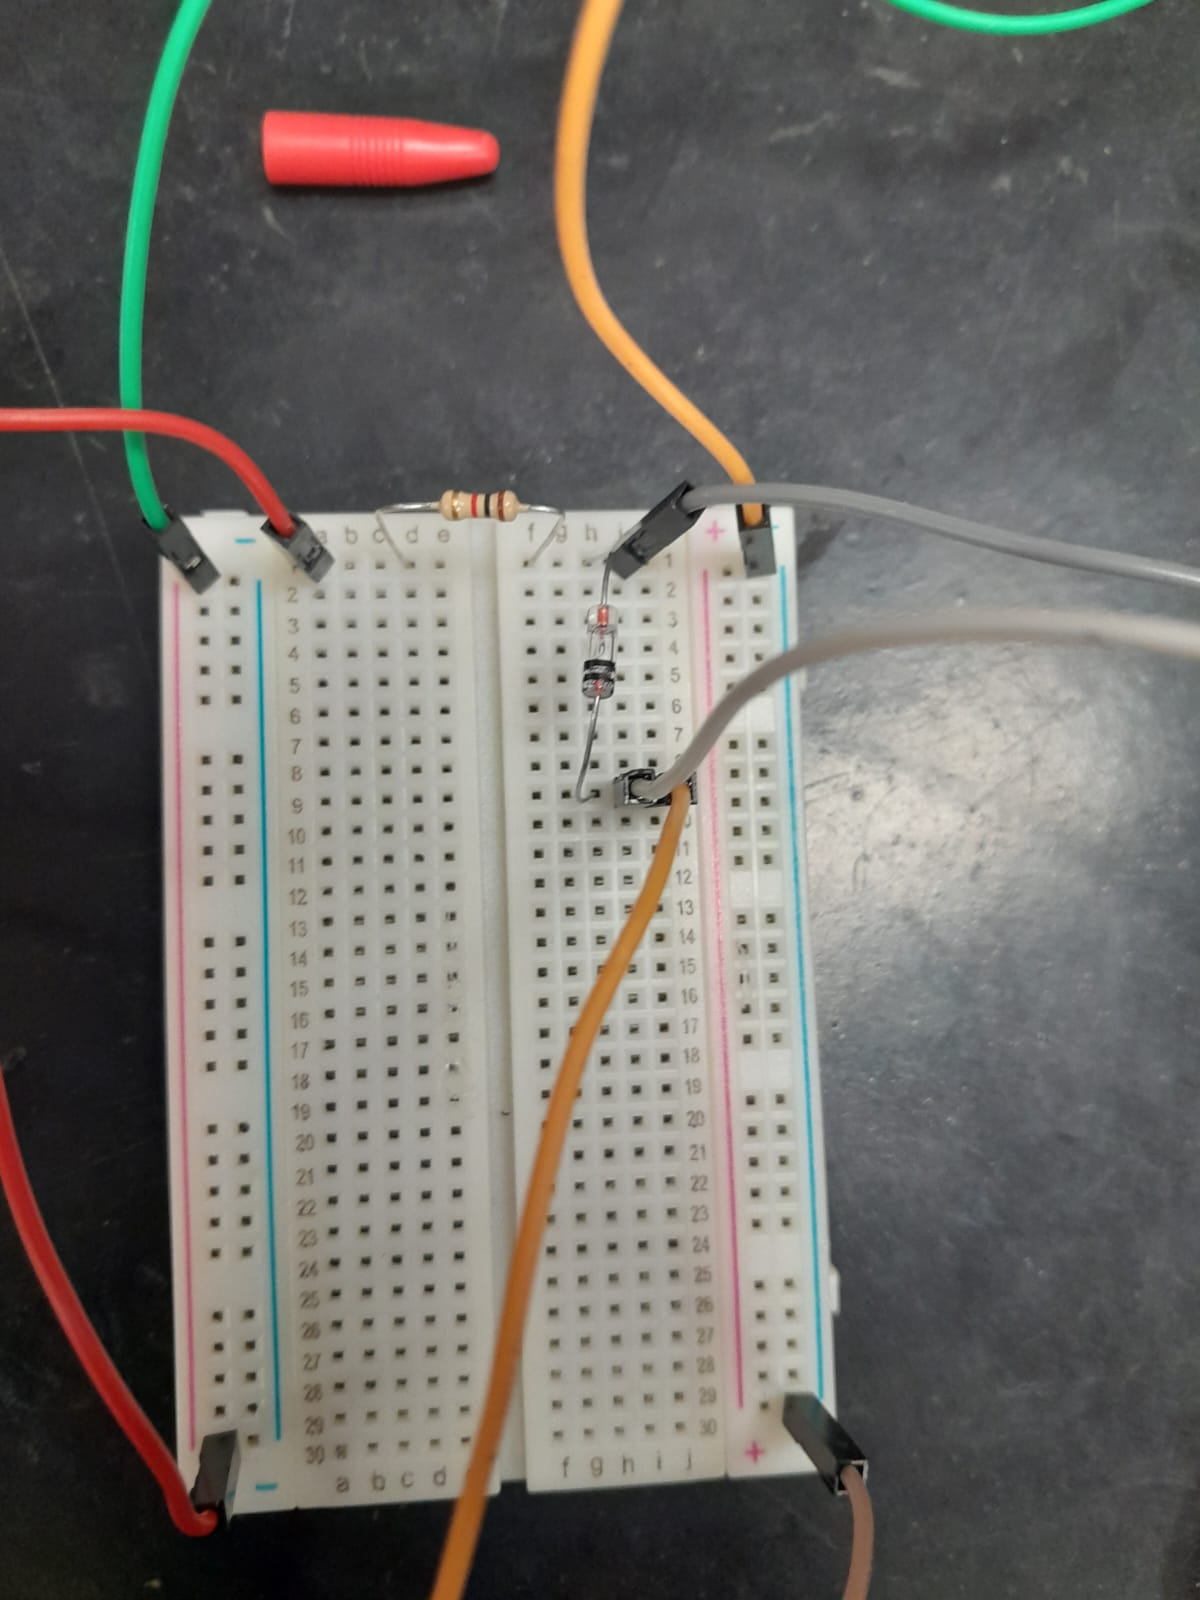
\includegraphics[width=7cm]{imagenes/proto1.jpg}
    \caption{Circuito de medición con diodo}
\end{figure}

\begin{figure}[H]
    \centering
    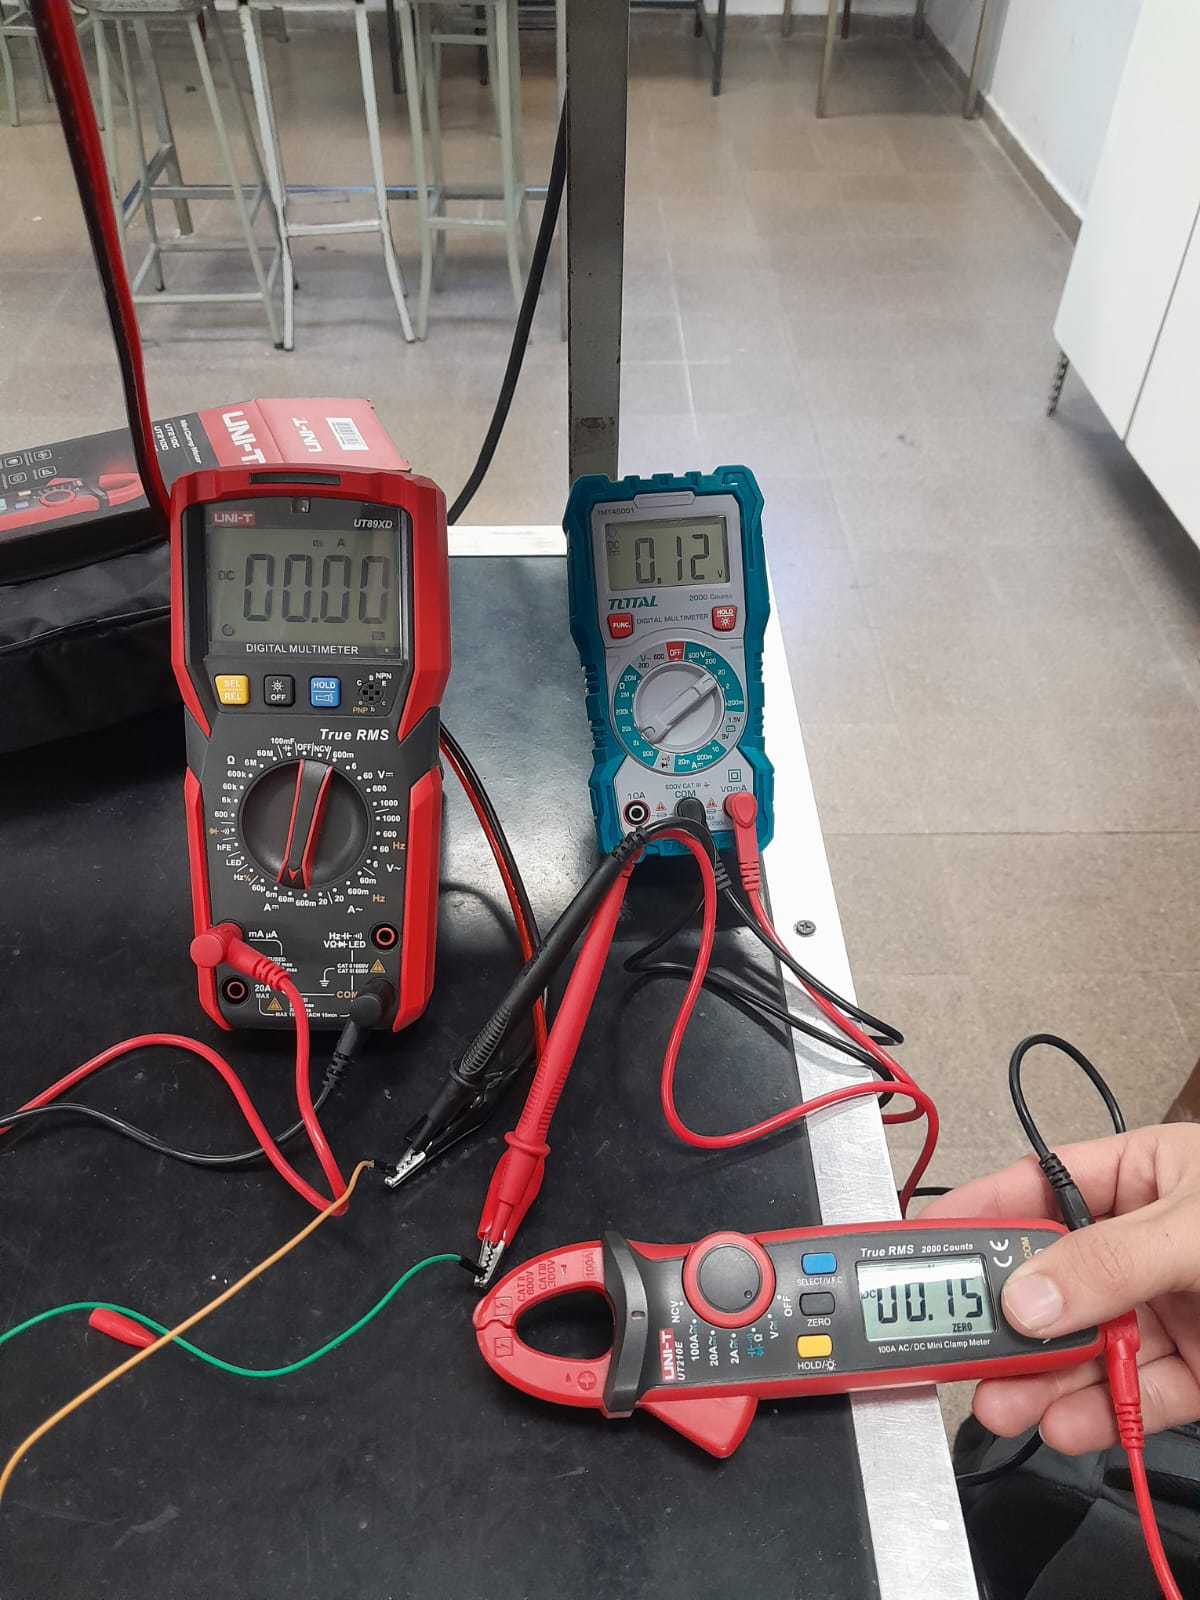
\includegraphics[width=7cm]{imagenes/elementos.jpg}
    \caption{Disposición de elementos}
\end{figure}


\subsection*{Tabla de mediciones Silicio}

\begin{table}[H]
\centering
\caption{Mediciones de laboratorio}
\begin{tabular}{|c|c|c|c|c|c|c|c|c|c|c|c|c|c|c|}
\hline
\textbf{V1 (V)} & 0 & 0.1 & 0.3 & 0.4 & 0.45 & 0.5 & 0.55\\
\hline
\textbf{VD} & 0 & 0.15 & 0.34 & 0.42 & 0.45 & 0.5 & 0.53\\
\hline
\textbf{ID} & 0 & 0 & 0 & 0 & 0 & 0.01m & 0.05m\\
\hline
\end{tabular}
\end{table}

\begin{table}[H]
\centering
\caption{Mediciones de laboratorio}
\begin{tabular}{|c|c|c|c|c|c|c|c|c|c|c|c|c|}
\hline
\textbf{V1 (V)}  & 0.6 & 0.65 & 0.7 & 1 & 3 & 5\\
\hline
\textbf{VD}  & 0.54 & 0.55 & 0.57 & 0.6 & 0.69 & 0.72\\
\hline
\textbf{ID}  & 0.08m & 0.1m & 0.17m & 0.41 & 2.49m & 4.28m\\
\hline
\end{tabular}
\end{table}


\subsection*{Tabla de mediciones Germanio}

\begin{table}[H]
\centering
\caption{Mediciones de laboratorio}
\begin{tabular}{|c|c|c|c|c|c|c|c|c|c|c|c|c|c|c|}
\hline
\textbf{V1 (V)} & 0 & 0.1 & 0.3 & 0.4 & 0.45 & 0.5 & 0.55\\
\hline
\textbf{VD} & 0 & 83.8m & 160m & 183m & 193m & 0.203 & 0.211\\
\hline
\textbf{ID} & 0 & 0.01m & 0.13m & 0.21m & 0.25m & 0.29m & 0.33m\\
\hline
\end{tabular}
\end{table}

\begin{table}[H]
\centering
\caption{Mediciones de laboratorio}
\begin{tabular}{|c|c|c|c|c|c|c|c|c|c|c|c|c|}
\hline
\textbf{V1 (V)}  & 0.6 & 0.65 & 0.7 & 1 & 3 & 5\\
\hline
\textbf{VD}  & 0.218 & 0.228 & 0.236 & 0.275 & 0.469 & 0.619 \\
\hline
\textbf{ID}  & 0.37m & 0.42m & 0.47m & 0.71m & 2.52m & 4.4m\\
\hline
\end{tabular}
\end{table}



% Gráfica de ID vs V1 para el diodo de germanio y silicio
\begin{figure}[H]
    \centering
    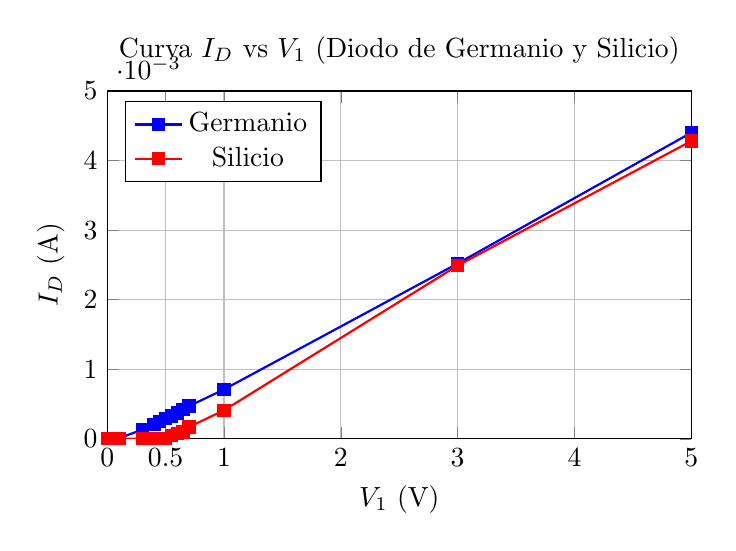
\begin{tikzpicture}
        \begin{axis}[
            width=9cm,
            height=6cm,
            grid=major,
            xlabel={$V_1$ (V)},
            ylabel={$I_D$ (A)},
            title={Curva $I_D$ vs $V_1$ (Diodo de Germanio y Silicio)},
            xmin=0, xmax=5,
            ymin=0, ymax=0.005,
            xtick={0,0.5,1,2,3,4,5},
            ytick={0,0.001,0.002,0.003,0.004,0.005},
            legend pos=north west
        ]
        % Diodo de Germanio (azul)
        \addplot[
            color=blue,
            mark=square*,
            thick
        ] coordinates {
            (0,0)
            (0.1,0.00001)
            (0.3,0.00013)
            (0.4,0.00021)
            (0.45,0.00025)
            (0.5,0.00029)
            (0.55,0.00033)
            (0.6,0.00037)
            (0.65,0.00042)
            (0.7,0.00047)
            (1,0.00071)
            (3,0.00252)
            (5,0.0044)
        };
        % Diodo de Silicio (rojo)
        \addplot[
            color=red,
            mark=square*,
            thick
        ] coordinates {
            (0,0)
            (0.1,0)
            (0.3,0)
            (0.4,0)
            (0.45,0)
            (0.5,0.00001)
            (0.55,0.00005)
            (0.6,0.00008)
            (0.65,0.0001)
            (0.7,0.00017)
            (1,0.00041)
            (3,0.00249)
            (5,0.00428)
        };
        \legend{Germanio, Silicio}
        \end{axis}
    \end{tikzpicture}
    \caption{Gráfica de $I_D$ en función de $V_1$ para los diodos de germanio (azul) y silicio (rojo)}
\end{figure}

% Gráfica de VD vs V1 para el diodo de germanio
\begin{figure}[H]
    \centering
    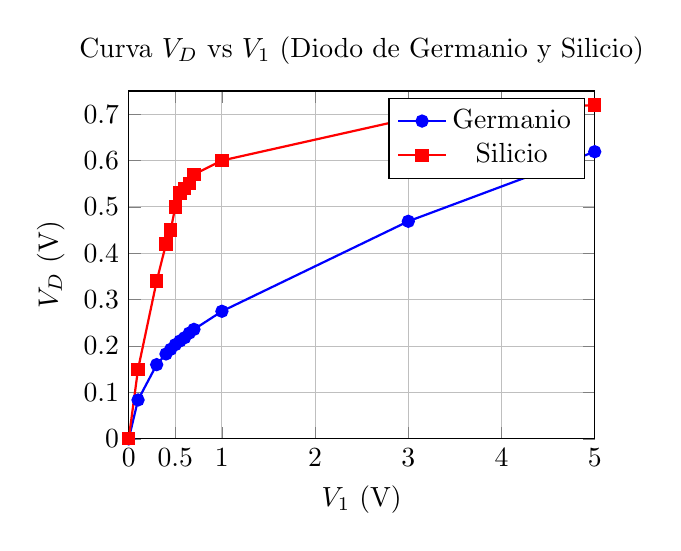
\begin{tikzpicture}
        \begin{axis}[
            width=7.5cm,
            height=6cm,
            grid=major,
            xlabel={$V_1$ (V)},
            ylabel={$V_D$ (V)},
            title={Curva $V_D$ vs $V_1$ (Diodo de Germanio y Silicio)},
            xmin=0, xmax=5,
            ymin=0, ymax=0.75,
            xtick={0,0.5,1,2,3,4,5},
            ytick={0,0.1,0.2,0.3,0.4,0.5,0.6,0.7}
        ]
        % Diodo de Germanio (azul)
        \addplot[
            color=blue,
            mark=*,
            thick
        ] coordinates {
            (0,0)
            (0.1,0.0838)
            (0.3,0.16)
            (0.4,0.183)
            (0.45,0.193)
            (0.5,0.203)
            (0.55,0.211)
            (0.6,0.218)
            (0.65,0.228)
            (0.7,0.236)
            (1,0.275)
            (3,0.469)
            (5,0.619)
        };
        % Diodo de Silicio (rojo)
        \addplot[
            color=red,
            mark=square*,
            thick
        ] coordinates {
            (0,0)
            (0.1,0.15)
            (0.3,0.34)
            (0.4,0.42)
            (0.45,0.45)
            (0.5,0.5)
            (0.55,0.53)
            (0.6,0.54)
            (0.65,0.55)
            (0.7,0.57)
            (1,0.6)
            (3,0.69)
            (5,0.72)
        };
        \legend{Germanio, Silicio}
        \end{axis}
    \end{tikzpicture}
    \caption{Gráfica de $V_D$ en función de $V_1$ para los diodos de germanio (azul) y silicio (rojo)}
\end{figure}


\subsection*{Presentar}

\begin{itemize}
    \item Fotografía con la disposición de los elementos del circuito e instrumentos.
    \item Sobre una misma gráfica, representar ambas curvas bien identificadas.
\end{itemize}

\begin{figure}[H]
    \centering
    %\includegraphics[width=0.7\textwidth]{curva_lab_comparada.jpg}
    \caption{Curva comparada 1N4007 vs. 1N60}
\end{figure}

\[ 
\]
\subsection{Comportamiento del diodo en función de la temperatura}
\section*{Objetivo}
El objetivo de esta actividad es simular la curva corriente-voltaje (I-V) de un diodo 1N3198 a distintas temperaturas y observar cómo varía:
\begin{itemize}
    \item El voltaje de conducción.
    \item La corriente de fuga inversa.
\end{itemize}

\subsection{Paso 1: Armado del circuito}
Se realizó el circuito mostrado en la Figura 1, compuesto por una fuente de tensión DC, una resistencia de 1 k$\Omega$ y un diodo 1N3198.

% AQUÍ VA LA IMAGEN DEL CIRCUITO EN LTSPICE
\begin{figure}[H]
    \centering
    %\includegraphics[width=0.7\textwidth]{ruta/circuito_ltspice.png}
    \caption{Circuito básico del diodo en polarización directa.}
\end{figure}

\subsection{Paso 2: Configuración de la simulación}

\subsection*{Fuente de tensión}
Se configuró la fuente de tensión V1 para realizar un barrido DC desde 0 V hasta 0.8 V en pasos de 0.01 V, utilizando el siguiente comando:
\begin{verbatim}
.dc V1 0 0.8 0.01
\end{verbatim}

\subsection*{Temperaturas}
Se añadió la siguiente directiva SPICE para realizar simulaciones a tres temperaturas distintas (20°C, 100°C y 125°C):
\begin{verbatim}
.step temp list 20 100 125
\end{verbatim}

\subsection{Paso 3: Ejecución de la simulación}

La simulación se ejecutó en LTspice. Se observaron las curvas corriente-voltaje del diodo para las distintas temperaturas especificadas. A continuación, se muestran las curvas resultantes.

% AQUÍ VA LA IMAGEN DE LOS RESULTADOS DE LA SIMULACIÓN (CURVA I-V)
\begin{figure}[H]
    \centering
    %\includegraphics[width=0.7\textwidth]{ruta/resultados_simulacion.png}
    \caption{Curvas I-V del diodo a diferentes temperaturas.}
\end{figure}

\subsection{Paso 4: Análisis de resultados}

Se observa que, a medida que aumenta la temperatura:
\begin{itemize}
    \item El voltaje de conducción del diodo disminuye. Es decir, el diodo comienza a conducir a un menor voltaje.
    \item La corriente de fuga inversa aumenta significativamente.
\end{itemize}

Este comportamiento concuerda con las características físicas del diodo de silicio, cuyo umbral de conducción se reduce con la temperatura debido al aumento de la generación térmica de pares electrón-hueco.

\subsection*{Conclusión}
A través de la simulación se pudo verificar cómo varía la curva característica I-V del diodo con la temperatura. Se comprobó que el aumento de la temperatura reduce el voltaje de conducción y aumenta la corriente de fuga inversa, tal como predice la teoría.